Standardisieren Sie den folgenden Stackautomaten für die Sprache
$L=\{\texttt{a}^n\texttt{b}^m\mid n\ge m\}$ als Vorbereitung
darauf, die Grammatik abzulesen.
\begin{center}
\def\h{2}
\def\r{0.35}
\def\punkt#1#2{({(#1)*\h},{(#2)*\h})}
\def\zustand#1#2{
	\draw #1 circle[radius=\r];
	\node at #1 {#2};
}
\def\akzeptierzustand#1#2{
	\draw #1 circle[radius={\r-0.05}];
}
\def\pfeil#1#2{
	\draw[->,shorten >= 0.35cm,shorten <= 0.35cm] #1 -- #2;
}
\begin{tikzpicture}[>=latex,thick]
\coordinate (q0) at (0,0);
\coordinate (q1) at (\h,0);
\zustand{(q0)}{$q_0$}
\zustand{(q1)}{$q_1$}
\pfeil{(q0)}{(q1)}
\end{tikzpicture}
\end{center}

\begin{loesung}
\end{loesung}
